The PE module includes a \textbf{is\_pe} variable that verifies whether the malware is an executable file. 
\\
\\
Moreover, the PE module includes both \textbf{DLL} and \textbf{characteristics} variables that verify whether the malware is a dynamic library file. As a matter of fact, every executable file links to a dynamic library, hence a dynamic library file may not be executable but an executable file is always dynamic link library.
\\
\\
The ELF module includes a \textbf{machine} variable that keeps the properties of machine code and assembly code of the malware and verifies whether the malware is an output file. In our case, the assembly is X86 and the machine code is 64-bit. Hence we choose to verify \textbf{EM\_X86\_64} which means output file with X86 assembly coding and 64-bit machine language.
\\
\\

\begin{yaracode}


import "pe"
import "elf"


rule elf_64
{
    condition:
        elf.machine==elf.EM_X86_64
}

rule is_dll
{
    condition:
        pe.characteristics & pe.DLL
}

rule is_pe
{
    condition:
        pe.is_pe
}


\end{yaracode}
The output when the rule is applied to our malware is like the following
\\

\begin{figure}[H]

    \centering
    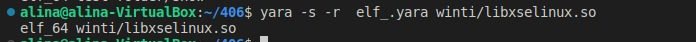
\includegraphics[width=\textwidth]{pe_elf.jpg}
    \caption{Detecting type of the malware by PE and ELF module}
    \label{fig:file_pe_elf}
    
\end{figure}
This output indicates that the malware is neither executable, nor a dynamically linked library. Rather the malware is an output file, which we have verified earlier in the classic process as well, with output \ref{fig:file_type}
\\